\documentclass[11pt]{article}
\usepackage[margin=1in]{geometry}
\usepackage[T1]{fontenc}
\usepackage[utf8]{inputenc}
\usepackage{lmodern}
\usepackage{booktabs}
\usepackage{amsmath}
\usepackage{graphicx}
\usepackage{xcolor}
\usepackage[hidelinks]{hyperref}
\usepackage{natbib}
\setcitestyle{authoryear,round}
\newcommand{\pending}{\textcolor{red}{\textbf{[pending]}}}

\title{When a Model Fabricates, It Stops Reading the Prompt:\\ Cheap Claim-Level Hallucination Detection from Attention}
\author{Anonymous submission}
\date{}

\begin{document}
\maketitle

\begin{abstract}
Claim-level hallucination detection for long-form LLM output remains hard and expensive: on the
MUCH benchmark the strongest published method, Claim-Conditioned Probability (CCP), reaches
0.77 ROC-AUC while costing more compute than generation itself. We show that when an LLM states a
false claim, its attention measurably \emph{retrieves less from the prompt} and \emph{leaks more onto
the attention sink}, an effect consistent across four models and visible at every depth. GRASP
turns this into a detector: three interpretable statistics (grounding, sink leakage, dispersion)
from a few label-free-selected heads per layer, plus the token probabilities the model already
produced, fed to a small gradient-boosted classifier. On MUCH's human-annotated test split GRASP
reaches 0.924 ROC-AUC against CCP's 0.770 (0.943 vs 0.811 against human consensus labels), wins
on every model and claim type, and costs 33--38\% of generation time on a T4 where CCP costs
192--430\% on the same hardware. On RAGTruth, trained with labels from the target benchmark it
beats CCP and the pre-trained UHeads of \citet{shelmanov-etal-2025-head} (0.827 vs 0.623 and
0.680); trained on MUCH plus two RAGTruth task types, it outperforms both on the held-out third
task (pooled 0.723 vs 0.623 and 0.680). Trained on a single benchmark and moved to a different
task family, it does not: there pre-trained UHeads transfer better. Training-free variants do not
beat CCP.
\end{abstract}

\section{Introduction}
LLMs state invented facts as fluently as true ones, so a safe deployment needs to know \emph{which}
claim to check, not merely that an answer is risky \citep{min-etal-2023-factscore}. MUCH
\citep{dentan2026muchmultilingualclaimhallucination} makes claim-level detection measurable at
scale: 4,873 long-form answers from four open models in four languages, segmented into 20,751
claims, with generated tokens and top-24 probabilities released. Its best baseline, CCP
\citep{fadeeva-etal-2024-fact}, filters token uncertainty through a natural-language-inference
model at every token. It is accurate (0.772 ROC-AUC) but costs more than generation.

We ask what the model's own attention reveals. Our first finding is mechanistic: across four
models, attention during a hallucinated claim is less grounded in the prompt and more often parked
on the attention sink (\S\ref{sec:mechanism}). Our second is practical: a small classifier on a
handful of such statistics, plus free token probabilities, beats CCP by a wide margin at a fraction
of its cost, and with diverse supervision it transfers to unseen task types better than a large
pre-trained detector. Our third is a set of explicit negative results: no zero-shot win across
benchmark families when trained on one benchmark, and no training-free win.

\textbf{Contributions.} (1) Evidence, consistent across four models and all depths, that hallucinated
claims show lower prompt grounding and higher sink leakage. (2) GRASP, an interpretable, cheap,
claim-level detector built on it. (3) An evaluation that keeps every choice on training data and
reports against GPT-4o and human labels, per model and claim type, across benchmarks, against CCP
and UHeads, with runtime measured on the same GPU. (4) An honest map of where it does not work.

\section{Related work}
\textbf{Probability-based} scores such as token likelihood and entropy are cheap but conflate lexical
and factual uncertainty; CCP \citep{fadeeva-etal-2024-fact} removes lexical variation with NLI at a
large cost. \textbf{Sampling-based} methods such as SelfCheckGPT \citep{manakul-etal-2023-selfcheckgpt}
and semantic entropy \citep{kuhn2023semanticuncertaintylinguisticinvariances} multiply cost and
miss consistent errors. \textbf{Internal-state probes} predict hallucination from hidden states
\citep{azaria2023internalstatellmknows,chen2024insidellmsinternalstates} or attention: Lookback
Lens \citep{chuang2024lookbacklensdetectingmitigating} uses the ratio of attention to context versus
generated text, SinkProbe \citep{binkowski2026attentionsinksinternalsignals} the sink mass, and RAUQ
\citep{vazhentsev2026efficienthallucinationdetectionllms} label-free head selection at sequence level.
\citet{lee2026meanshift} find that simple regularised probes suffice in a paired setting. Closest to
us, UHeads \citep{shelmanov-etal-2025-head} train a transformer head on attention and probability
features for claim-level detection. GRASP differs in using three interpretable statistics from a few
label-free-selected heads and a small tree model; we compare to UHeads directly.

\begin{table}[t]
\centering\small
\begin{tabular}{lcccc}
\toprule
Method & Granularity & Signal & Extra passes & Labels \\
\midrule
CCP \citep{fadeeva-etal-2024-fact} & claim & probabilities + NLI & NLI per token & no \\
SelfCheckGPT \citep{manakul-etal-2023-selfcheckgpt} & sentence & sample agreement & $N$ samples & no \\
Semantic entropy \citep{kuhn2023semanticuncertaintylinguisticinvariances} & sequence & sample meaning & $N$ samples & no \\
SAPLMA \citep{azaria2023internalstatellmknows} & sentence & hidden states & none & yes \\
Lookback Lens \citep{chuang2024lookbacklensdetectingmitigating} & span & context/self attention ratio & none & yes \\
RAUQ \citep{vazhentsev2026efficienthallucinationdetectionllms} & sequence & attention to previous token & none & no \\
UHeads \citep{shelmanov-etal-2025-head} & claim & attention + probabilities & transformer head & yes \\
\textbf{GRASP} & claim & grounding, sink, dispersion + probs & one replay & yes (free variant: no) \\
\bottomrule
\end{tabular}
\caption{Related detectors.}
\label{tab:related}
\end{table}

\section{Method}
\subsection{Per-token attention signals}
The generated tokens are replayed once through the model. For generated token $t$ and a kept head,
with attention row $a_t$ over positions $0..t$ (position 0 is the sink, $1..P{-}1$ the prompt),
we compute grounding to the prompt $G_t$, sink leakage $S_t$ and dispersion $D_t$:
\begin{align}
G_t &= \frac{\sum_{j=1}^{P-1} a_{t,j}}{\sum_{j\ge 1} a_{t,j}}, \qquad S_t = a_{t,0},\\
D_t &= \frac{-\sum_{j\ge1} \tilde a_{t,j}\log \tilde a_{t,j}}{\log |\{j\ge1\}|},
\end{align}
where $\tilde a$ is the non-sink row renormalised, and the row used is the one that produced $t$.

\subsection{Label-free head selection}
Per layer we keep the $k{=}4$ heads whose $G$ varies most across tokens on 200 unlabelled answers
from the same model; a head with near-constant $G$ cannot discriminate.

\subsection{Claim features and classifier}
Layers are pooled into 8 relative-depth bins so models of different depth share one feature space.
For each bin, kept head and signal, a claim's content tokens give the mean, max, min and a
saliency-weighted mean of the per-(layer, head) z-scored value (384 features). Seven features come
from the token probabilities already produced (chosen-token surprisal, entropy, top-1 probability,
top-1/top-2 gap) and two from claim length. A gradient-boosted tree classifier (31 leaves, 800
rounds) predicts the label. \textbf{GRASP-free} averages, without labels, the per-model rank of
mid-depth minimum grounding and of token surprisal and entropy, with signs fixed a priori.

\section{Experimental setup}
\textbf{Benchmarks.} \emph{MUCH}: all 8 configurations (Llama-3.2-3B, Llama-3.1-8B, Gemma-3-4B,
Ministral-8B; temperature 0.7 and 1.0). Test is the 200 human-annotated answers (867 claims); train
the other 4,673 (19,884 claims). Following MUCH's evaluator we score against GPT-4o labels on
claims where GPT-4o and GPT-4.1 agree, and additionally against the two human annotators.
\emph{RAGTruth} \citep{niu-etal-2024-ragtruth}: Mistral-7B-Instruct responses to retrieval-augmented
QA, summarisation and data-to-text; claims from MUCH's segmenter, hallucinated if they overlap an
annotated span; 445 test responses (17,226 claims). \emph{AkimBio}: \pending{}.

\textbf{Protocol.} Every modelling choice was made by 5-fold cross-validation on training data,
grouped by answer and ranked by the \emph{mean of per-model} ROC-AUCs (pooled ROC can be inflated
by recognising the model, as hallucination rates range from 22\% to 54\%). Choices were frozen to a
file before any test split was read; evaluation rules for RAGTruth were written before its features
existed. MUCH's test split was read by an earlier version too; we report this.

\textbf{Baselines.} CCP as released by MUCH ($\delta{=}24$, $\sigma{=}8$, product aggregation),
reproduced at 0.775 / 0.643 ROC/PR (published 0.772 / 0.639), and re-run with MUCH's own code on
RAGTruth; token surprisal and entropy; UHeads via the authors' pre-trained claim heads, run on
identical claims, and retrained on our training data (\pending{}).

\textbf{Statistics.} 95\% CIs from 2,000 bootstrap resamples of answers; differences paired on
identical claims.

\section{Why it works: hallucinated claims are less grounded}
\label{sec:mechanism}
\begin{figure}[t]
\centering
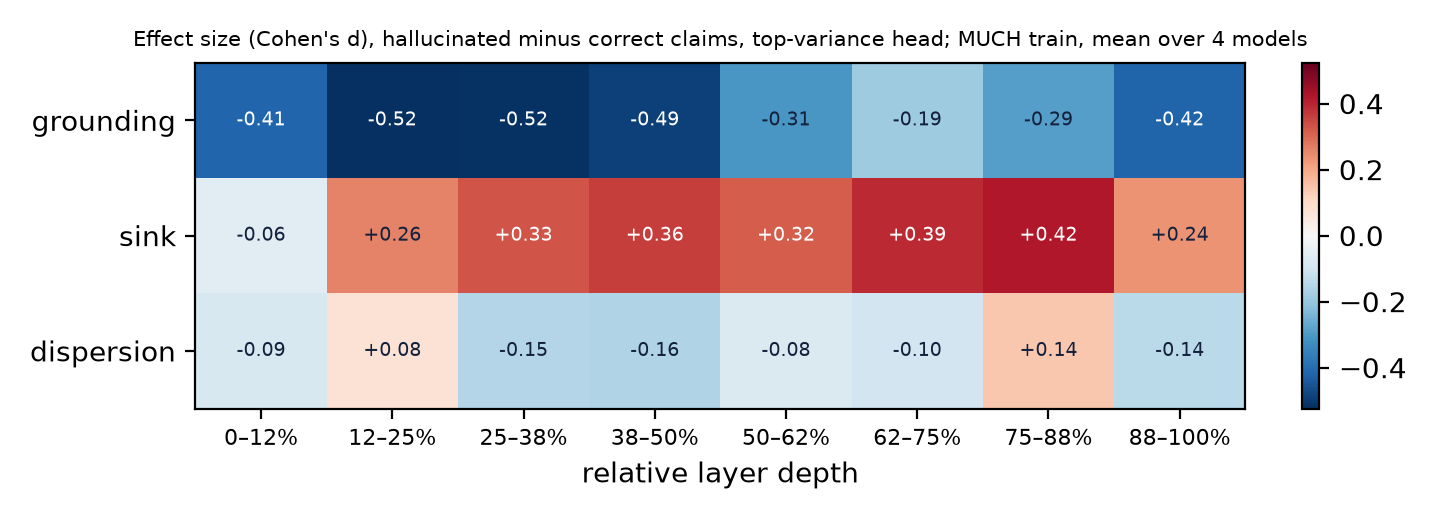
\includegraphics[width=\linewidth]{../results/figures/effect_size_signal_depth.png}
\caption{Effect size (Cohen's $d$) between hallucinated and correct claims for the mean signal over a
claim's content tokens, top-variance head, by relative depth; MUCH training claims, averaged over
four models. Blue: lower for hallucinated claims.}
\label{fig:effect}
\end{figure}
Figure~\ref{fig:effect} shows the raw signals before any classifier. For hallucinated claims,
grounding to the prompt is lower at every depth ($d\approx-0.4$ to $-0.5$, strongest in the
first half of the network), and sink leakage is higher from about 12\% depth onward
($d\approx+0.3$ to $+0.4$). Dispersion shows no consistent effect ($|d|<0.16$). When the model
fabricates, it reads less from what it was asked and parks more attention on the sink. A
permutation analysis of the trained classifier (Figure~\ref{fig:imp}) agrees: among attention
groups, sink leakage at 62--75\% depth contributes most, dispersion least. Token probabilities
carry the largest single share, and the attention groups are mutually redundant, so each looks
small alone. Together they lift cross-validated ROC from 0.771 (probabilities alone) to 0.866.
\begin{figure}[t]
\centering
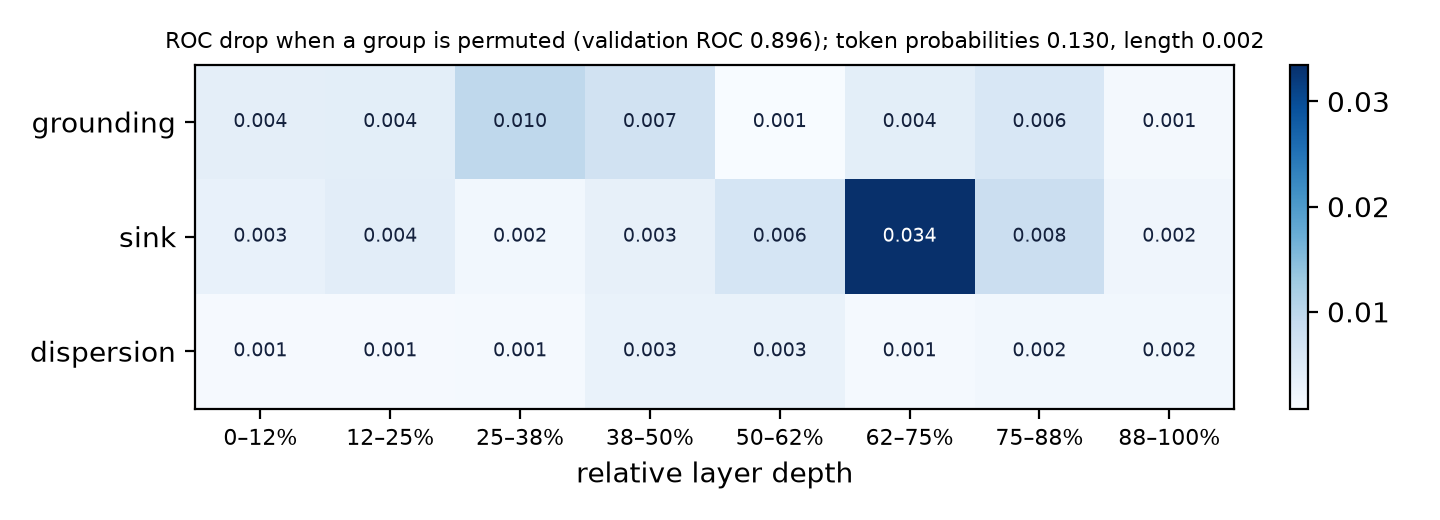
\includegraphics[width=\linewidth]{../results/figures/importance_signal_depth.png}
\caption{ROC drop when a feature group is permuted, GRASP trained on 80\% of MUCH training answers
and measured on the other 20\%.}
\label{fig:imp}
\end{figure}

\section{Results}
\subsection{MUCH}
\begin{table}[t]
\centering\small
\begin{tabular}{lccccc}
\toprule
 & \multicolumn{3}{c}{GPT-4o labels (867 claims)} & \multicolumn{2}{c}{human consensus (842)} \\
Method & ROC-AUC [95\% CI] & PR-AUC & TPR@10\% & ROC-AUC & $\Delta$ vs CCP \\
\midrule
CCP & 0.770 [0.724, 0.817] & 0.637 & 0.537 & 0.811 & -- \\
GRASP-free & 0.764 [0.713, 0.815] & 0.501 & 0.354 & 0.777 & $-$0.034 \\
\textbf{GRASP} & \textbf{0.924} [0.896, 0.948] & \textbf{0.845} & \textbf{0.790} & \textbf{0.943} & \textbf{+0.132} [+0.091, +0.178] \\
\bottomrule
\end{tabular}
\caption{MUCH human-annotated test split. GRASP's $\Delta$ROC vs CCP on GPT-4o labels: +0.154 [+0.110, +0.199].}
\label{tab:main}
\end{table}
GRASP beats CCP on every model (Gemma-3-4B 0.917 vs 0.726, Llama-3.1-8B 0.937 vs 0.831, Llama-3.2-3B
0.889 vs 0.767, Ministral-8B 0.897 vs 0.830; all paired CIs exclude zero) and against each human
annotator separately (0.928 and 0.939 vs 0.802 and 0.808). Across five runs on different 90\% samples
of the training answers, test ROC is $0.916\pm0.003$ (human labels $0.936\pm0.004$). At response level
(any hallucination in the answer) it reaches 0.911 vs 0.762.

\textbf{Claim types.} GRASP wins on numbers and dates (0.960 vs 0.867), named entities (0.937 vs 0.779)
and other claims (0.865 vs 0.659), with the largest gain where CCP is weakest.

\textbf{Unseen model.} Trained on three models and scored on the fourth, GRASP beats CCP on three and
trails on Llama-3.2-3B (0.759 vs 0.767).

\subsection{RAGTruth}
\begin{table}[t]
\centering\small
\begin{tabular}{llcc}
\toprule
Training data & Method & ROC-AUC [95\% CI] & $\Delta$ROC vs CCP \\
\midrule
-- & CCP & 0.623 [0.602, 0.644] & -- \\
authors' data & UHead (pre-trained) & 0.680 [0.649, 0.708] & +0.057 [+0.029, +0.083] \\
MUCH only & GRASP + rank normalisation & 0.639 [0.617, 0.659] & +0.015 [$-$0.011, +0.042] \\
MUCH + other 2 RAGTruth tasks & GRASP (held-out task, pooled) & \textbf{0.723} [0.700, 0.746] & \textbf{+0.099} [+0.071, +0.129] \\
RAGTruth train & GRASP & \textbf{0.827} [0.803, 0.849] & \textbf{+0.203} [+0.177, +0.233] \\
\bottomrule
\end{tabular}
\caption{RAGTruth test, claim level (UHead row on its 17,181 covered claims).}
\label{tab:rag}
\end{table}
Table~\ref{tab:rag} separates three regimes. With RAGTruth's own labels GRASP beats CCP by 0.20 and
the pre-trained UHead by 0.15. Trained on MUCH alone it reaches only CCP's level, even after a
label-free per-domain rank normalisation selected by MUCH leave-one-model-out (0.808 $\to$ 0.819
held-out ROC on MUCH). There the pre-trained UHead, trained on far more varied data, transfers better.
With moderately diverse supervision (MUCH plus two RAGTruth task types), GRASP beats both on the
held-out task: QA 0.795 (UHead 0.644), summaries 0.737 (0.676), data-to-text 0.679 (0.702, CI of the
difference crosses zero); pooled +0.043 over UHead [+0.009, +0.077]. In RAGTruth's
retrieval-augmented setting, attention matters more than probabilities: in training cross-validation
attention alone gives 0.785, probabilities alone 0.619, both 0.801.

\subsection{Comparison with UHeads}
\label{sec:uheads}
On MUCH's Llama-3.1-8B test claims, the authors' pre-trained Llama head scores 0.570, against 0.831
for CCP, 0.883 for GRASP trained on the other three models and 0.937 in-domain. The head is weak on
MUCH even on training claims (oriented ROC 0.526) while the same code is sensible on RAGTruth, which
points to a mismatch with MUCH's very short claims. A same-data comparison with UHeads retrained on
our training splits is \pending{}.

\subsection{Runtime and abstention}
On Tesla T4s, GRASP's extraction pass costs 33--38\% of measured generation time; MUCH's CCP, timed on
the same hardware, costs 235--430\% on MUCH's models and 192\% on RAGTruth answers. For selective
answering, withholding the 30\% of claims GRASP rates riskiest leaves 7.2\% hallucinated among the rest
(CCP: 14.7\%; base rate 26.4\%).

\section{Limitations}
GRASP is supervised: its wins need labels from the target setting, or at least diverse related
supervision; trained on one benchmark and moved to a different task family it does not beat a large
pre-trained head. Training-free variants do not beat CCP at claim or response level. MUCH's test
split was read more than once (all choices frozen on training data beforehand), and further reads of
RAGTruth test were made for additional analyses. Evaluation covers two benchmarks with released claim
labels and five generator models; a third benchmark is \pending{}. RAGTruth's span labels miss many
hallucinations \citep{yu2026rt4chart}, depressing absolute scores. CCP and generation were timed on
different sample generations (compared per token). RAGTruth responses were replayed through
Mistral-7B-Instruct-v0.1, assumed to be the generator version.

\section{Conclusion}
Hallucinated claims leave a consistent trace in attention: less grounding in the prompt, more
leakage onto the sink. Reading that trace from a few heads, together with the probabilities the
model already computed, gives a claim-level detector that beats CCP and pre-trained UHeads when
trained with relevant labels, at a sixth of CCP's cost, and transfers to unseen task types when the
supervision is diverse. Transfer across very different task families without such supervision
remains open.

\bibliographystyle{plainnat}
\bibliography{../papers/references}
\end{document}
